\documentclass[11pt]{report}
\usepackage{mathrsfs,graphicx}
\begin{document}

\noindent
George Weigt

\noindent
Homework \#1

\bigskip
\noindent
{\bf 1a.} Derive the Laplace transform for the following function.
$$f(t)=tu(t)$$

\bigskip
\noindent
We do not have to worry about the unit step function $u(t)$ because all
it does is ensure that $f(t) = 0$ for $t<0$ which is required by the
Laplace transform
(Ogata p. 13.)
That leaves us with $t$ and according to the table on p. 17
the Laplace transform of $t$ is $s^{-2}$.
Hence
$${\mathscr L}[tu(t)]={1\over s^2}$$

\bigskip
\noindent
{\bf 1b.} Derive the Laplace transform for the following function.
$$f(t)=\sin\omega t\,u(t)$$

\bigskip
\noindent
Again, we can ignore $u(t)$.
From the table on p. 17 we obtain
$${\mathscr L}[\sin\omega t\,u(t)]={\omega\over s^2+\omega^2}$$

\bigskip
\noindent
{\bf 2.} Derive the Laplace transform for the following function.
$$f(t)=e^{-at}\cos\omega t\,u(t)$$

\bigskip
\noindent
The unit step function $u(t)$ is implicit in the Laplace transform tables.
By the table on p. 17 we have
$$F(s)={\mathscr L}[\cos\omega t\,u(t)]={s\over s^2+\omega^2}$$
Then by the complex shifting theorem (Lecture 2, p. 12) we have
$${\mathscr L}[e^{-at}\cos\omega t\,u(t)]=F(s+a)={s+a\over (s+a)^2+\omega^2}$$

\newpage

\noindent
{\bf 3a.} Use {\sc matlab} to find the Laplace transform of the following
function.
$$f(t)=5te^{-2t}\sin(4t+60^\circ)$$

\bigskip
\noindent
For this problem I used a free web-based applet instead of {\sc matlab}.

\bigskip
\noindent
Input:
\begin{center}
\verb$5*t*exp(-2*t)*sin(4*t+pi/3)$
\end{center}

\bigskip
\noindent
Output:
$$-{5\sqrt3\over2((s+2)^2+16)}
-{5(2s+4)\left(-{\sqrt3(s+2)\over2}-2\right)\over((s+2)^2+16)^2}$$

\bigskip
\noindent
Screenshot:
\begin{center}
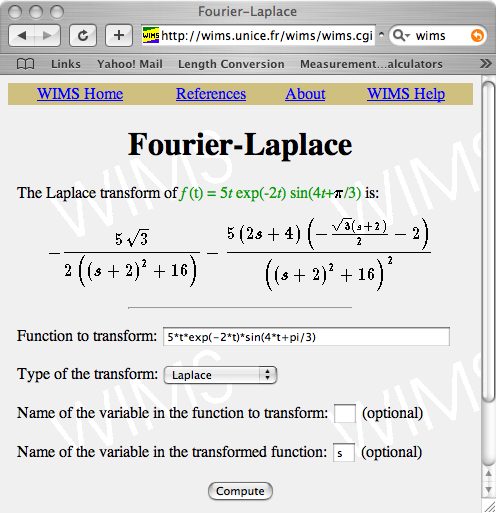
\includegraphics[scale=0.5]{images/laplace-tool.png}
\end{center}

\newpage

\noindent
{\bf 3b.} Use {\sc matlab} to find the inverse Laplace transform of the following
function.
$$G(s)={(s^2+3s+7)(s+2)\over(s+3)(s+4)(s^2+2s+100)}$$

\bigskip
\noindent
For this problem I used a free web-based applet instead of {\sc matlab}.

\bigskip
\noindent
Input:
\begin{center}
\verb$(s^2+3*s+7)*(s+2)/(s+3)/(s+4)/(s^2+2*s+100)$
\end{center}

\bigskip
\noindent
Output:
$$-{7\exp(-3t)\over103}
+{11\exp(-4t)\over54}
+{\exp(-t)
\left(4807\cos(3t\sqrt{11})-{4681\sqrt{11}\sin(3t\sqrt11)\over11}\right)
\over5562}$$

\bigskip
\noindent
Screenshot:
\begin{center}
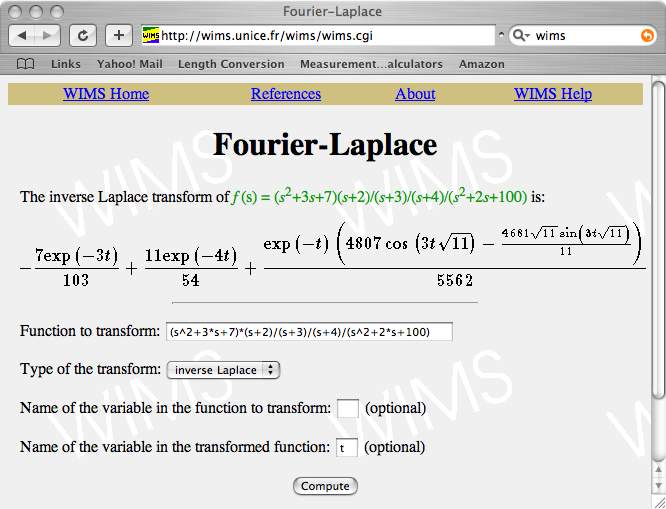
\includegraphics[scale=0.5]{images/inverse-laplace-tool.png}
\end{center}

\newpage

\noindent
{\bf 4.} Find the transfer function for the following differential
equation.
$${d^3y\over dt^3}+3{d^2y\over dt^2}+5{dy\over dt}+y
={d^3x\over dt^3}+4{d^2x\over dt^2}+6{dx\over dt}+8x$$

\bigskip
\noindent
It turns out that the transfer function is obtained using a simple pattern
involving the coefficients (Ogata p. 55.)
We have
$a_0,a_1,a_2,a_3=1,3,5,1$ and $b_0,b_1,b_2,b_3=1,4,6,8$.
Hence the transfer function is
$${Y(s)\over X(s)}={s^3+4s^2+6s+8\over s^3+3s^2+5s+1}$$

\bigskip
\noindent
{\bf 5.} Find the differential equation for the following transfer function.
$${Y(s)\over X(s)}={s+2\over s^3+8s^2+9s+15}$$

\bigskip
\noindent
The degree of the numerator polynomial is less than or equal to the degree of
the denominator polynomial so it is OK to use the coefficient trick
(Ogata p. 55.)
We have $a_0,a_1,a_2,a_3=1,8,9,15$ and $b_0,b_1=1,2$.
Hence the differential equation is
$${d^3y\over dt^3}+8{d^2y\over dt^2}+9{dy\over dt}+15y
={dx\over dt}+2y$$

\newpage

\noindent
{\bf 6. (B-2-11)} Find the inverse Laplace transform of
$$F(s)={s+1\over s(s^s+s+1)}$$

\bigskip
\noindent
Separating the numerator we have
$$F(s)={1\over s^2+s+1}+{1\over s(s^2+s+1)}$$
Let
$$F_1(s)={1\over s^s+s+1}$$
and let $\omega=1$ and $\zeta={1\over2}$.
Then
$$F_1(s)={\omega^2\over s^s+2\zeta\omega s+\omega^2}$$
Apply transform pair 22 (Ogata p. 18) to obtain
$${\mathscr L}^{-1}[F_1(s)]={2\over\sqrt3}e^{-t/2}\sin{\sqrt3t\over 2}$$
Let
$$F_2(s)={1\over s(s^s+s+1)}={\omega^2\over s(s^2+2\zeta\omega s+\omega^2)}$$
Apply transform pair 24 (Ogata p. 18) to obtain
$${\mathscr L}^{-1}[F_2(s)]=1-{2\over\sqrt3}e^{-t/2}\sin
\left({\sqrt3t\over2}+{\pi\over3}\right)$$
By the angle-sum relation we have
$${\mathscr L}^{-1}[F_2(s)]=1-{2\over\sqrt3}e^{-t/2}
\left({1\over2}\sin{\sqrt3t\over2}+{\sqrt3\over2}\cos{\sqrt3t\over2}\right)
=1-e^{-t/2}\left({1\over\sqrt3}\sin{\sqrt3t\over2}+\cos{\sqrt3t\over2}\right)
$$
Hence
$${\mathscr L}^{-1}[F(s)]={\mathscr L}^{-1}[F_1(s)]+{\mathscr L}^{-1}[F_2(s)]=
1+e^{-t/2}\left(
{1\over\sqrt3}\sin{\sqrt3t\over2}-\cos{\sqrt3t\over2}\right)$$

\newpage

\noindent
{\bf 7a. (B-2-13a)} Find the inverse Laplace transform of the following
function.
$$F(s)={6s+3\over s^2}$$

\bigskip
\noindent
Separate the numerator to obtain
$$F(s)={6\over s}+{3\over s^2}$$
Apply transform pairs 2 and 3 to obtain
$$f(t)=(6+3t)u(t)$$

\bigskip
\noindent
{\bf 7b. (B-2-13b)} Find the inverse Laplace transform of the following
function.
$$F(s)={5s+2\over(s+1)(s+2)^2}$$

\bigskip
\noindent
The partial fraction expansion of $F(s)$ is
$$F(s)={A\over s+1}+{B\over s+2}+{C\over(s+2)^2}$$
We have
$$A=\left[(s+1){5s+2\over(s+1)(s+2)^2}\right]_{s=-1}=-3$$
$$B={1\over(2-1)!}\left[{d\over ds}
\left((s+2)^2{5s+2\over(s+1)(s+2)^2}\right)\right]_{s=-2}=3$$
$$C=\left[(s+2)^2{5s+2\over(s+1)(s+2)^2}\right]_{s=-2}=8$$
We have
$$F(s)=-{3\over s+1}+{3\over s+2}+{8\over(s+2)^2}$$
Hence
$$f(t)=-3e^{-t}+3e^{-2t}+8te^{-2t}$$

\end{document}
